\documentclass[../../Rapport RayTracer]{subfiles}

\begin{document}
	\label{packageMultithreading}
	
	Le package multithreading contient les trois classes qui sont utilisées pour le multithreading de notre ray tracer:
	\begin{description}
		\item [ThreadsTaskList] Maintient la liste des tâches à calculer par les threads
		\item [TileTask] Représente une tâche à calculer par un thread
		\item [TileThread] Classe implémentant l'interface Runnable permettant de créer les threads
	\end{description}
	
	\begin{figure}[h!]
		\adjustbox{center}{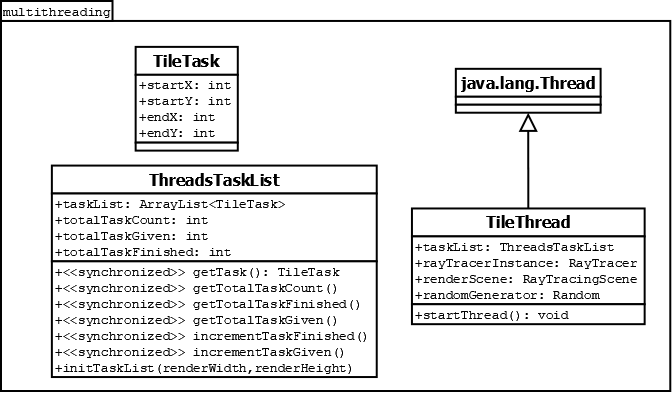
\includegraphics[width=\textwidth]{diagrammes/package_multithreading.png}}
		
		\caption{Diagramme du package multithreading}
		\label{packageMultithreadingFigure}
	\end{figure}
	\FloatBarrier
	
\end{document}